\section{Eilenberg--Steenrod 公理}
\sourcepage{169--170}
我们为特定空间类，即多面体，定义了同调群。历史上它们最先出现，后来各种推广定义适用于更一般的空间。这些同调理论有许多共同特点，在多面体上都给出与单纯同调相同的结果。

同调理论的多样性促使 Eilenberg 和 Steenrod 将其公理化。他们提炼出共同的关键性质，并证明这些性质在多面体类上完全刻画同调群。

这里不复述完整公理化方法，也不证明刻画定理，可参阅 [ES52]。我们只列出七条公理，另加处理非紧致空间所需的一条公理。下一节验证单纯同调满足它们。

\entry{定义}{3.5.1}设 $\mathcal A$ 为拓扑空间偶 $(X,A)$（$A\subset X$）的一个类，满足：
\begin{enumerate}[label=(\arabic*)]
\item 若 $(X,A)\in\mathcal A$，则 $(X,X),(X,\varnothing),(A,A),(A,\varnothing)$ 也属于此类。
\item 若 $(X,A)\in\mathcal A$，则 $(X\times I,A\times I)$ 也属于此类。
\item 存在单点空间 $P$，使 $(P,\varnothing)\in\mathcal A$。
\end{enumerate}
称 $\mathcal A$ 为同调理论的一个\textbf{容许空间类}（admissible class）。

\entry{定义}{3.5.2}若 $\mathcal A$ 容许，则其上的一个\textbf{同调理论}由三个函数组成：
\begin{enumerate}[label=(\arabic*)]
\item 对每个整数 $p$ 和偶 $(X,A)$ 指定阿贝尔群 $H_p(X,A)$。
\item 对每个连续映射 $h:(X,A)\to(Y,B)$ 指定同态 $(h_*)_p:H_p(X,A)\to H_p(Y,B)$。
\item 对每个偶指定同态 $(\partial_*)_p:H_p(X,A)\to H_{p-1}(A)$，其中 $A$ 表示 $(A,\varnothing)$。
\end{enumerate}
它们须满足下列公理，涉及的偶均在 $\mathcal A$ 中。仍省略诱导映射的维数下标。

\entry{公理}{1}恒等映射诱导恒等同态。

\entry{公理}{2}$(k\circ h)_*=k_*\circ h_*$。

\sourcepage{171}
\entry{公理}{3}若 $f:(X,A)\to(Y,B)$，则边界的自然性成立：
\[
\begin{array}{ccc}
H_p(X,A)&\xrightarrow{f_*}&H_p(Y,B)\\
\downarrow\scriptstyle\partial_*&&\downarrow\scriptstyle\partial_*\\
H_{p-1}(A)&\xrightarrow{(f|_A)_*}&H_{p-1}(B).
\end{array}
\]

\entry{公理}{4（正合公理）}序列
\[
\cdots\to H_p(A)\xrightarrow{i_*}H_p(X)\xrightarrow{\pi_*}H_p(X,A)
\xrightarrow{\partial_*}H_{p-1}(A)\to\cdots
\]
正合，其中 $i:A\to X$、$\pi:X\to(X,A)$ 为包含。

回顾：$h,k:(X,A)\to(Y,B)$ 同伦，指存在连续 $F:(X\times I,A\times I)\to(Y,B)$，满足 $F(x,0)=h(x)$、$F(x,1)=k(x)$。

\entry{公理}{5（同伦公理）}若 $h\simeq k$，则 $h_*=k_*$。

\entry{公理}{6（切除公理）}给定 $(X,A)$，若 $U$ 在 $X$ 中开，$\overline U\subset\Int A$，且 $(X\setminus U,A\setminus U)$ 容许，则包含诱导同构
\[
H_p(X\setminus U,A\setminus U)\cong H_p(X,A).
\]

\entry{公理}{7（维数公理）}若 $P$ 为单点空间，则 $p\ne0$ 时 $H_p(P)=0$，而 $H_0(P)=\Z$。

\entry{公理}{8（紧支撑公理）}若 $\alpha\in H_p(X,A)$，则存在容许偶 $(X_0,A_0)$，其中 $X_0,A_0$ 紧致，使 $\alpha$ 属于包含诱导同态 $H_p(X_0,A_0)\to H_p(X,A)$ 的像。

两空间均紧致的偶称为\textbf{紧致偶}。也可把维数公理改为 $H_0(P)=G$，其中 $G$ 为固定阿贝尔群，得到“以 $G$ 为系数的同调”。目前仍使用整数系数。

维数公理似乎最无害、最不有趣，但在某种意义上恰好相反。公理提出后，人们发现了类似同调的新理论，例如微分拓扑的配边理论和向量丛理论中的 K 理论。它们的发明目的与同调群最初的目的很不同，却共享许多形式性质，尤其满足除维数公理外的 Eilenberg--Steenrod 公理。

\sourcepage{172}
如今称这种理论为\textbf{非普通同调理论}（extraordinary homology theory），或\textbf{广义同调理论}（generalized homology theory）。它与普通同调的区别是，单点空间也可能在许多维数上有非零同调。这说明数学中反复出现的现象：为一种目的建立的理论，会产生远超创始者预想的后果。

以下定义用于习题 1。

\entry{定义}{3.5.3}下列阿贝尔群及同态的交换图称为\textbf{辫形图}（braid）：
\begin{center}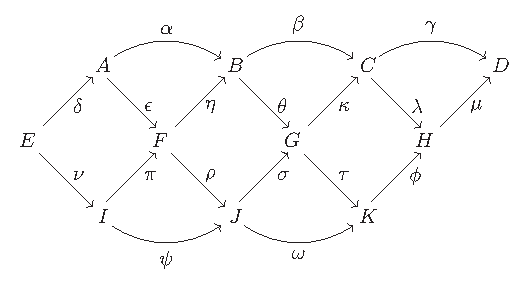
\includegraphics[width=114mm]{figures/3-5-braid.pdf}\end{center}
图中有四列，形如相互叠合的正弦曲线。前三列为
\[
\left.\begin{aligned}
E&\to A\to B\to G\to K,\\
E&\to I\to J\to G\to C\to D,\\
A&\to F\to J\to K\to H\to D,
\end{aligned}\right\}\tag{$*$}
\]
第四列为 $I\to F\to B\to C\to H$。若四列均正合，称为\textbf{正合辫形图}。

\entry{引理}{3.5.4（辫形图引理）}若 $(*)$ 的三列正合，且复合 $I\to F\to B$ 为零，则整个辫形图正合。

以下定义用于习题 3。

\entry{定义}{3.5.5}设 $X=X_1\cup X_2$，$A=X_1\cap X_2$。若 $(X_1,A)$、$(X,X_2)$ 容许，且包含 $(X_1,A)\to(X,X_2)$ 诱导同调同构，则称 $(X_1,X_2)$ 为给定同调理论的\textbf{可切除空间对}（excisive couple）。

\sourcepage{173--174}
\subsection*{习题}
\begin{enumerate}
\item \begin{enumerate}[label=(\alph*)]
\item 若定义 3.5.3 的辫形图正合，证明存在同构 $\Lambda:(\ker\omega)/(\operatorname{im}\psi)\to(\ker\beta)/(\operatorname{im}\alpha)$，定义如下：若 $\omega(j)=0$，选 $f$ 使 $\rho(f)=j$，令 $\Lambda(\{j\})=\{\eta(f)\}$。
\item 证明辫形图引理。
\end{enumerate}
\item 设 $X\supset A\supset B$，称 $(X,A,B)$ 为拓扑空间三元组，同调语境下默认上述嵌套关系。仅使用同调公理，证明三元组同调序列
\[
\cdots\to H_p(A,B)\xrightarrow{\pi}H_p(X,B)\xrightarrow{\eta}H_p(X,A)
\xrightarrow{\beta}H_{p-1}(A,B)\to\cdots
\]
正合，其中 $\pi,\eta$ 由包含诱导，$\beta$ 为复合 $H_p(X,A)\xrightarrow{\partial_*}H_{p-1}(A)\xrightarrow{i_*}H_{p-1}(A,B)$。假定各偶容许。［提示：证明 $H_p(A,A)=0$、$\eta\pi=0$，再用习题 1。］
\item 仅使用公理，按下列方法导出 Mayer--Vietoris 序列。
\begin{enumerate}[label=(\alph*)]
\item 设 $i:A\to X_1$、$j:A\to X_2$、$k:X_1\to X$、$\ell:X_2\to X$ 为包含，$\alpha:X_1\to(X_1,A)$、$\beta:X\to(X,X_2)$ 及 $\gamma:(X_1,A)\to(X,X_2)$ 也为包含，给出相应的长正合列同态。若 $(X_1,X_2)$ 可切除，按
\[
\begin{aligned}
\varphi(a)&=(i_*a,-j_*a),\\
\psi(x_1,x_2)&=k_*x_1+\ell_*x_2,\\
\theta(x)&=\partial_*\gamma_*^{-1}\beta_*(x)
\end{aligned}
\]
定义序列 $\cdots\to H_p(A)\xrightarrow{\varphi}H_p(X_1)\oplus H_p(X_2)\xrightarrow{\psi}H_p(X)\xrightarrow{\theta}H_{p-1}(A)\to\cdots$。其中 $\partial_*$ 为 $(X_1,A)$ 的边界同态。证明它正合，且对于连续映射诱导的同态自然。［提示：作图表追踪，从每隔三个位置就是同构的长正合列同态出发。］
\item 若 $X=|K|$，$X_1,X_2$ 为子复形的多胞体，证明它们对单纯同调可切除，且所得序列就是定理 3.4.1 的序列。
\item 假定 $(X_1,A)$、$(X,X_2)$ 容许。若 $\Int X_1$ 与 $\Int X_2$ 覆盖 $X$，且 $X_1$ 在 $X$ 中闭，证明此空间对对任何满足公理的同调理论都可切除。
\end{enumerate}
\end{enumerate}
